\renewcommand{\arraystretch}{1.5}
\begin{CJK*}{UTF8}{gbsn}
\begin{figure}[h]
  \centering
  \begin{tabular}{m{7cm}m{8cm}}
  \toprule
  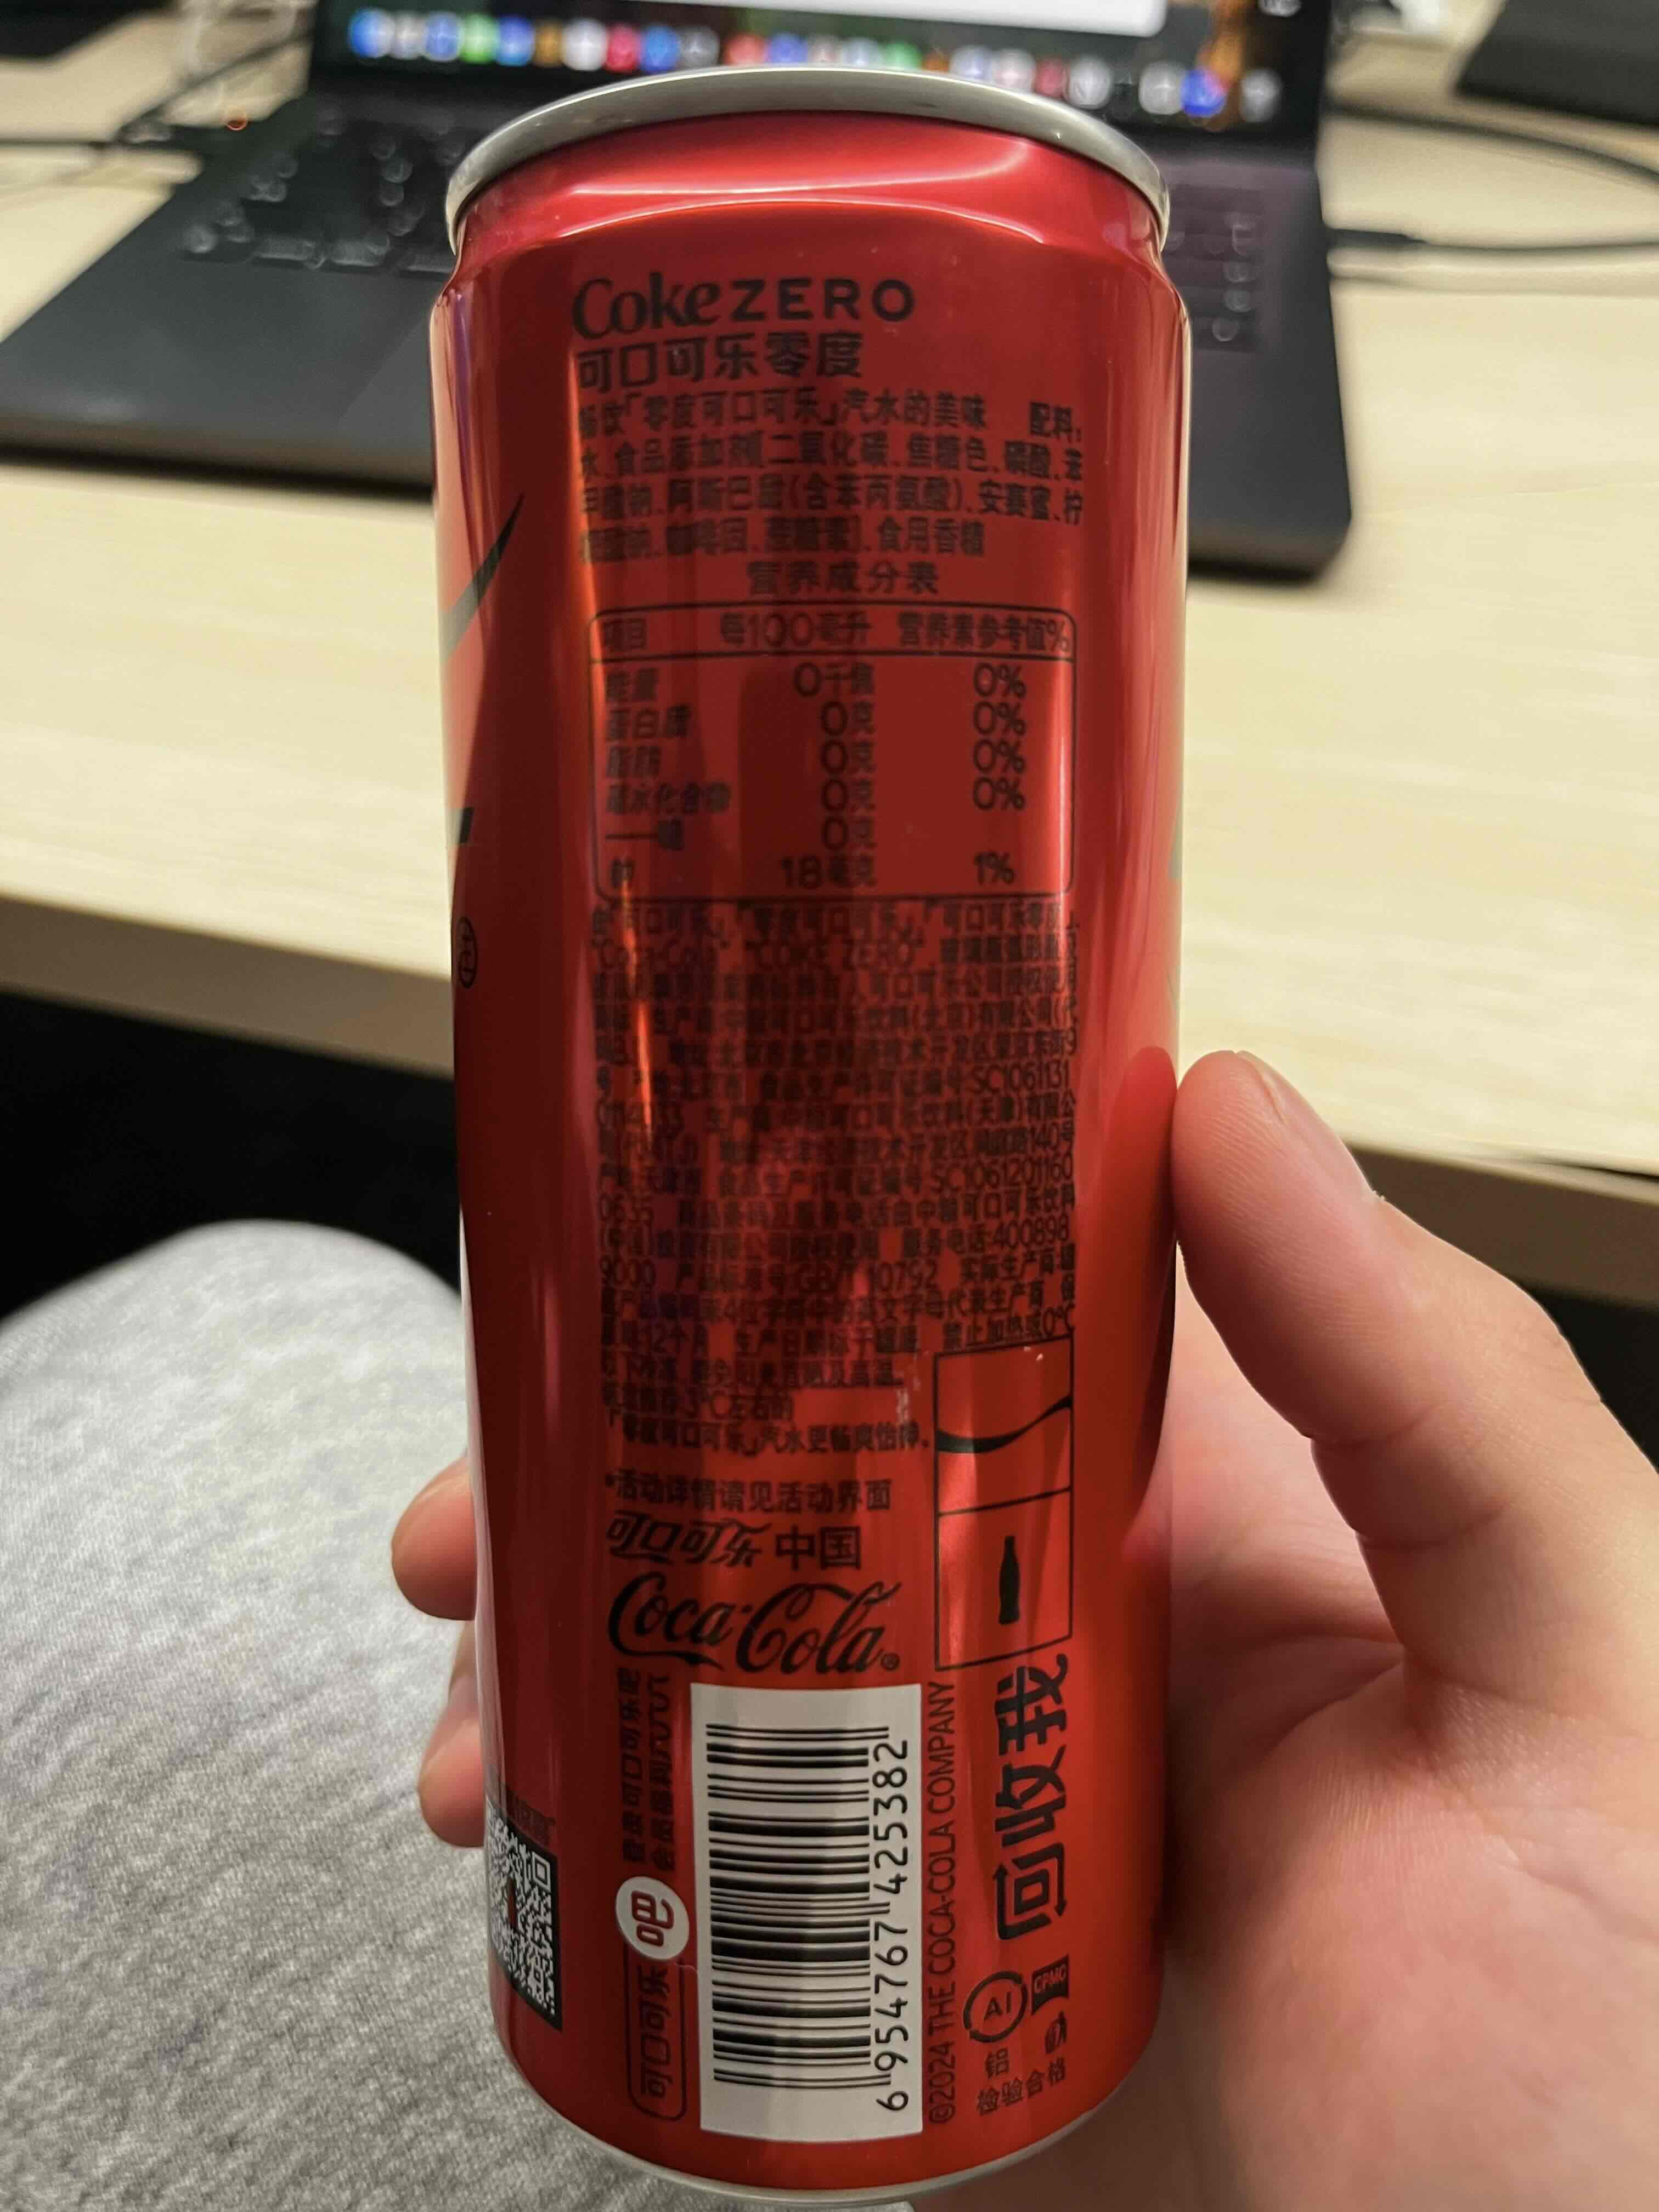
\includegraphics[width=7cm]{figures/example/example2.jpeg} & 
  {\textbf{Instruction:} 这瓶可乐喝10罐会摄入多少克钠？\par
  \textbf{\mimovlrl{}:} \texttt{<think>...</think>}要计算喝10罐可口可乐零度时摄入的钠量，需按以下步骤分析：  
  \begin{enumerate}
      \item \textbf{步骤1：明确营养成分表信息}
    从图片中“营养成分表”可知：\textbf{每100毫升}该饮料中，钠的含量为 \textbf{18毫克}。  
      \item \textbf{步骤2：确定单罐饮料容量（行业常见规格）}
    可口可乐零度的罐装规格通常为 \textbf{330毫升/罐}（这是饮料行业的常见罐装容量，若实际容量不同需以产品标注为准，此处默认330ml）。
     \item \textbf{步骤3：计算单罐钠含量}
    单罐（330ml）中钠的含量 = 每100ml钠含量 × 单罐容量 ÷ 100  
    即：$ 18\ \text{毫克/100ml} × 330\ \text{ml} ÷ 100 = 59.4\ \text{毫克} $  
    \item \textbf{步骤4：计算10罐钠总量} 
    10罐钠总量 = 单罐钠含量 × 10  
    即：$ 59.4\ \text{毫克} × 10 = 594\ \text{毫克} $ 
  \end{enumerate}
  \par
  因此，喝10罐该款可口可乐零度，约摄入 \textbf{594毫克} 钠。  } \\
  \hline
  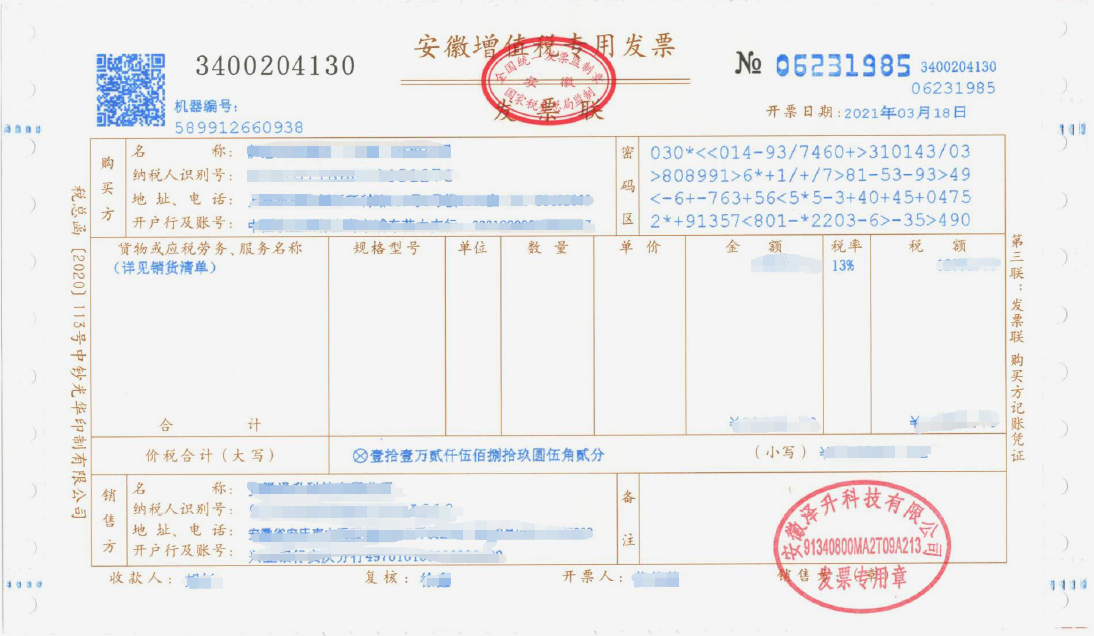
\includegraphics[width=7cm]{figures/example/example3.png} & 
  {\textbf{Instruction:} 该发票缺失的税额应该是多少？
\par
  \textbf{\mimovlrl{}:} \texttt{<think>...</think>}要计算该发票的税额，需结合\textbf{税率}和\textbf{价税合计金额}来推导： 
  \begin{enumerate}
      \item \textbf{步骤1：明确关键信息}
    - 发票税率：$13\%$（发票中“税率”栏显示）  
    - 价税合计金额（大写）：壹拾壹万贰仟伍佰捌拾玖圆伍角贰分，对应小写为 \textbf{112589.52元}
    \item \textbf{步骤2：税额的计算逻辑}  
    发票税额 = 价税合计金额 × （1 - 税率）× 税率   （即：总价价税合计 = 不含税金额 + 税额 → 税额 = 价税合计 × 税率 ÷ (1 + 税率) ）  
    \end{enumerate}
    设不含税金额为 $\ X $ ，则：  
    $ X + X×13\% = 112589.52 $
    $ X×1.13 = 112589.52 $  
    $ X = 112589.52 ÷ 1.13 = 99636.74 $ 元【不含税金额】  
    
    税额 = 不含税金额 × 税率 =  99636.74 × 13\% = 12952.78 元  
} \\
  \bottomrule
  \end{tabular}
\caption{Example of \mimovlrl{} solving complex OCR problems with reasoning.}
\label{fig:case2}
\end{figure}
\end{CJK*}
\renewcommand{\arraystretch}{1}

\clearpage
